% ═══════════════════════════════════════════════════════════════════════
\section{Calculer le PageRank : la méthode des puissances}
% ═══════════════════════════════════════════════════════════════════════

\begin{frame}{Algorithme 4.1 --- Méthode des puissances}
  \small \texttt{np.linalg.eig} calcule toutes les valeurs et tous les
  vecteurs propres d'une matrice pleine : inutilisable. Le théorème 4.6
  suggère plutôt d'appliquer $G$ de façon répétée.
  \begin{Algo}{Algorithme 4.1 --- Méthode des puissances pour le PageRank}
    \small Données : $A$ creuse, $\vec E$, $\beta$, une tolérance
    $\varepsilon>0$.
    \begin{enumerate}
      \item $\vec w_0=\frac1N\,\vec e$ (la loi uniforme).
      \item Pour $k=1,2,\dots$ :
        $\displaystyle \vec w_k = \beta A\vec w_{k-1}
        +\frac{\beta s_{k-1}+1-\beta}{N}\,\vec e$, où
        $s_{k-1}=\vec E^{\mathsf T}\vec w_{k-1}$.
      \item S'arrêter si $d_1(\vec w_k,\vec w_{k-1})<\varepsilon$ ; renvoyer
        $\vec w_k$.
    \end{enumerate}
  \end{Algo}
  \small
  \begin{itemize}
    \item Étape 2 = $G\vec w_{k-1}$, puisque $\vec e^{\mathsf T}\vec w=1$ ;
      $s$ est la masse sur les pages sans lien.
    \item Coût : le produit $A\vec w$, proportionnel au nombre de liens.
    \item $d_1(\vec x,\vec y)=\sum|x_i-y_i|$ : la taxi-distance du
      chapitre 2, dans $\R^N$.
  \end{itemize}
\end{frame}

\begin{frame}[fragile]{Programme 4.9 --- La méthode des puissances}
  \begin{columns}[T]
    \begin{column}{0.95\textwidth}
\begin{lstlisting}
def pagerank(liens, N, beta=0.85, tol=1e-8):
    """Méthode des puissances, sans construire G."""
    A = matrice_transition(liens, N)  # creuse
    sans_sortie = (A.sum(axis=0) == 0)  # le vecteur E
    w = np.ones(N) / N                  # départ : loi uniforme
    for k in range(1, 1000):
        s = w[sans_sortie].sum()        # le produit E^T w
        w_suiv = beta * (A @ w) + (beta*s + 1 - beta) / N
        if np.abs(w_suiv - w).sum() < tol:  # d_1
            return w_suiv, k
        w = w_suiv

q, k = pagerank(liens3, 7)     # 93 itérations
\end{lstlisting}
    \end{column}
  \end{columns}
  \small On retrouve le PageRank du mini-web 3. Ajouter un nombre à un
  vecteur l'ajoute à chaque composante : le terme en $\vec e$, sans
  construire $\vec e$.
\end{frame}

\begin{frame}{Théorème 4.8 --- Retour au théorème de Banach}
  \small Le théorème 4.6 ne dit pas combien d'itérations faire, et n'a été
  démontré que dans le cas diagonalisable. Banach donne une preuve
  complète, avec une estimation de l'erreur.
  \begin{Enonce}{Théorème 4.8 --- La matrice Google est une contraction}
    Soit $\Delta$ l'ensemble des vecteurs de probabilités de $\R^N$, muni
    de $d_1$. Pour tous $\vec x,\vec y\in\Delta$,
    \[
      d_1(G\vec x,G\vec y)\leq\beta\,d_1(\vec x,\vec y).
    \]
  \end{Enonce}
  \begin{AuTableau}
    \footnotesize $\vec z=\vec x-\vec y$ vérifie $\vec e^{\mathsf T}\vec z=0$,
    donc $G\vec z=\beta B\vec z$. Puis
    $\sum_i|\sum_j b_{ij}z_j|\leq\sum_j|z_j|\sum_i b_{ij}=\sum_j|z_j|$
    (coefficients positifs, colonnes de somme $1$).
  \end{AuTableau}
\end{frame}

\begin{frame}{Le PageRank, point fixe d'une contraction}
  \small
  \begin{itemize}
    \item $(\Delta,d_1)$ est complet : une suite de Cauchy de $\Delta$ a des
      composantes de Cauchy, donc convergentes, et la limite a encore des
      composantes positives de somme $1$.
    \item Banach (forme générale) : un unique point fixe $\vec q$, et la
      méthode converge quel que soit le départ --- sans Perron--Frobenius.
    \item Majoration de l'erreur :
      $d_1(\vec w_k,\vec q)\leq\frac{\beta^k}{1-\beta}\,d_1(\vec w_0,\vec w_1)$ ;
      en partant de $\vec w_{k-1}$ :
      $d_1(\vec w_k,\vec q)\leq\frac{\beta}{1-\beta}\,d_1(\vec w_{k-1},\vec w_k)$.
      Au critère d'arrêt, l'erreur est inférieure à
      $\frac{\num{0.85}}{\num{0.15}}\,\varepsilon\approx\num{5.7}\,\varepsilon$.
    \item Le nombre d'itérations ne dépend pas de la taille du Web. Comme
      $d_1\leq2$ sur $\Delta$ : $d_1(\vec w_k,\vec q)\leq2\beta^k$ ; pour
      $10^{-8}$ avec $\beta=\num{0.85}$, il suffit de $k\geq118$.
    \item Majoration pessimiste : le programme s'arrête après $93$
      itérations ; Page rapportait qu'une cinquantaine suffisaient sur des
      centaines de millions de liens.
  \end{itemize}
\end{frame}

\begin{frame}{Remarque 4.3 --- Le rôle de la seconde valeur propre}
  \begin{Rem}{Remarque 4.3}
    \small
    \begin{itemize}
      \item La vitesse est gouvernée par $|\lambda_2|$, le plus grand
        module des valeurs propres de $G$ autres que $1$ ; on démontre que
        $|\lambda_2|\leq\beta$ (cohérent avec le théorème 4.8).
      \item Mini-web 3 : égalité, $G$ a la valeur propre $-\num{0.85}$,
        héritée du $-1$ de $A$ (l'aller-retour $6\leftrightarrow7$).
      \item $\beta$ joue un double rôle : compromis fidélité /
        téléportation (tableau 4.3), et vitesse de convergence. Avec
        $\beta=\num{0.99}$ : environ $\num{1900}$ itérations pour la même
        précision.
    \end{itemize}
  \end{Rem}
  \small PageRank n'est qu'un critère parmi d'autres, et sa mise en œuvre
  chez Google n'a jamais été entièrement publiée. Mais l'idée sert
  ailleurs : citations scientifiques, équipes sportives, réseaux
  alimentaires --- chaque fois, un vecteur propre de valeur propre $1$.
\end{frame}

\begin{frame}{Pour la classe 4.4 --- Classer, une activité pour la classe}
  \begin{Classe}{Classer, une activité pour la classe}
    \small
    \begin{itemize}
      \item Un petit réseau de quatre ou cinq pages au tableau ; les élèves
        prédisent un classement (la plupart comptent les liens entrants).
      \item On simule l'internaute aléatoire avec un dé : une trentaine de
        clics par équipe ; on compare les fréquences à la prédiction.
      \item Un réseau bien choisi, comme celui de la figure 4.1, où une page
        qui reçoit peu de liens devance une page qui en reçoit autant,
        lance une discussion : que veut dire « être important » dans un
        réseau ?
      \item En Technico-sciences : calculer $A\vec p$ au tableur
        (multiplication matricielle).
    \end{itemize}
  \end{Classe}
\end{frame}

\begin{frame}{Note historique 4.4 --- Larry Page (né en 1973)}
  \footnotesize
  \begin{columns}[T]
    \begin{column}{0.25\textwidth}
      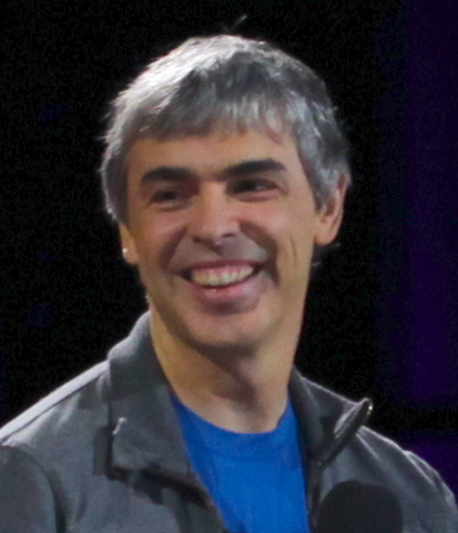
\includegraphics[width=\linewidth]{larry-page.jpg}\\
      {\scriptsize\color{gray}En 2014. Photo : Steve Jurvetson,
      CC BY 2.0, Wikimedia Commons.}
    \end{column}
    \begin{column}{0.72\textwidth}
      \begin{itemize}
        \item Né à East Lansing (Michigan) ; ses deux parents enseignent
          l'informatique. Doctorat à Stanford en 1995 (Terry Winograd) ;
          il y rencontre Sergey Brin.
        \item Analogie avec les citations : un article souvent cité, surtout
          par des articles importants, est important. Le robot du projet
          BackRub télécharge les liens du Web dès 1996.
        \item « The PageRank Citation Ranking » (1999) ; jeu de mots entre
          son nom et la page web. Brevet de Stanford, licence exclusive à
          Google.
        \item Septembre 1998 : Google, dans un garage de Menlo Park ; il
          abandonne son doctorat. PDG jusqu'en 2001, puis de 2011 à 2015 ;
          Alphabet jusqu'en 2019.
      \end{itemize}
    \end{column}
  \end{columns}
\end{frame}
